
\chapter{Evaluation}


In this section we will take a retrospective look at the tool and its achievements. We observe some benchmarks ran against competitors as well as measure how well Gentoo has performed given the expected pre-requisites as set out earlier in this thesis. We will also attempt to given a qualitative evaluation of how well it has performed, given initial user feedback (beyond the quantitative analysis). \\

\section{Metrics of success}

To appropriately judge the success of the extension, we must have some quantifiable metrics, described below

\begin{enumerate}
	\item \textbf{Time to vulnerability} - As mentioned in \ref{limitations}, measuring the total time taken to perform a scan in this human driven context is unfair; the tool does not set a boundary on total scans unlike an automated scanner does. Measuring time taken is however a useful metric, so in order to not completely circumvent using time, another more appropriate metric is suggested - \emph{time to vulnerability}. This will be measured as the total number of seconds taken from the moment a scan is initiated (the user clicks the visual cue given by the tool), until the scan is finished. A scan may finish under two circumstances: a vulnerability has been successfully reported or detected (this may happen at the first attempt by the user, or at a later try when the tool has fuzzed some inputs during the Action Replay phase), or when the tool reports it could not find a vulnerability. These 2 conditions are bounded in terms of possible time taken, allowing the total time to be measured.
	
	\item \textbf{Interaction volume} - A metric that is sometimes found when evaluating automated scanners  is that of bytes sent and received by the application \cite{stateOfArtAutomatedBlackBoxWebAppVulnTesting}. This quantifies the impact the tool has when stressing the website by fuzzing inputs. The smaller this metric is, the more efficiently the tool is performing its job, by detecting vulnerabilities with fewer web requests sent.
	
	\item \textbf{Number of replays needed} - A similar metric to interaction volume, this number measures how many 'replays' are required by the tool to successfully detect a vulnerability. Both of these metrics measure the efficiency of the tool in detecting vulnerabilities, but this metric more accurately tests the efficiency of the fuzzing engine provided by the tool. Ideally, the tool uses the inputs which are known to work with higher success rates first, and the more esoteric fuzzes would come last, when there is already a decreased likelihood of them working anyway. It also encourages the tool to only include meaningful and relevant fuzzing techniques per vulnerability type, otherwise the tool \emph{could} theoretically fuzz forever. The fewer number of replays needed by the tool in order to find a vulnerability, the better it is performing.
	
	%	\item \textbf{Recommendation to vulnerability conversion rate} - An automated scanner is often measured in terms of how many false positives it shows, because it is expected to either positively or negatively declare the existence of a vulnerability. This would be an unfair means of benchmarking this extension - 
\end{enumerate}


\section{Experiments}


\subsection{Test benches}
In order to test my tool during development, it is not necessary to build a vulnerable web application from scratch. Not only would this be time consuming (beyond the purposes of building a tool to exploit such an application), it would also bias the ensuing development of the extension so that it is tailored to successfully detect every injected vulnerability in the web application. Fortunately, there already exist tools dedicated to this purpose. \\

As previously mentioned, DVWA is a vulnerable web application written in PHP, using MySQL for database interactions \cite{dvwaSite}. This application contains a good selection of predefined vulnerabilities to test against:
\begin{multicols}{3}
	\begin{itemize}
		\item Brute Force Login
		\item Command Execution
		\item CSRF
		\item File Inclusion
		\item SQL Injection
		\item Upload Vulnerability
		\item XSS	
	\end{itemize}
\end{multicols}

Another existing tool is WebGoat \cite{webgoatIntro, webgoatGithub}, supported by OWASP. This is an actively supported project by the open source community, and also contains a healthy amount of potential vulnerabilities for developers to test against:

\begin{multicols}{3}
	\begin{itemize}
		\item 	Access Control Flaws
		\item 	AJAX Security
		\item 	Authentication Flaws
		\item 	Buffer Overflows
		\item 	Code Quality
		\item 	Concurrency
		\item 	XSS
		\item 	Improper Error Handling
		\item 	Injection Flaws
		\item 	Denial of Service
		\item 	Insecure Communication
		\item 	Insecure Configuration
		\item 	Insecure Storage
		\item 	Malicious Execution
		\item 	Parameter Tampering
		\item 	Session Management Flaws
		\item 	Web Services
		\item 	Admin Functions
	\end{itemize}
\end{multicols}

Similarly to the above, there exist more testing tools of this kind, such as WackoPicko \cite{wackoPickoGithub} and HacmeBank \cite{hacmeBankMcAfee}. A more extensive list of existing applications of this kind has been produced by OWASP \cite{owaspVulnerableWebAppsList}. For the purposes of the experiments in this project, I will test against DVWA, WebGoat and WackoPicko, in order, as needed per vulnerability. This provides a good variety of implementations of vulnerabilities to test against; if the tool successfully finds the targeted vulnerabilities in these applications then it is likely to do well in other contexts.

\subsection{Test methodology}
The main method of testing my extension is to pit my extension against other existing automated vulnerability scanners. Some potential candidate scanners include \emph{OWASP ZAP} \cite{owaspZapPage}, \emph{w3af} \cite{w3af} and \emph{burpsuite} \cite{burpSuitePage}. All the scanners will analyse the aforementioned vulnerable applications used in testing. To avoid the case where the produced extension overfits its scanning model to the test vulnerable applications, this experiment will include more applications from the OWASP vulnerable web apps list \cite{owaspVulnerableWebAppsList}, not previously used in testing. \\

Since the browser extension makes use of user input, it is important to test the application with people of different security backgrounds. This relies on adequate classification in this group by the person undertaking the test. There will be 3 proposed categories of user experience when testing the tool; advanced, intermediate and beginner. An advanced user is expected to be well versed in web security, and have had prior experience in diagnosing (perhaps exploiting) vulnerabilities. An intermediate user may be someone getting to grips with this area, perhaps a student who is only now learning about these concepts, but hasn't \emph{necessarily} got experience in detecting or exploiting vulnerabilities. Beginner users are expected to be web savvy, people who are acquainted with using browsers and web applications, but are not necessarily interested or knowledgeable in web security. It is hoped that enough data is gathered to be able to have at least 5 unique people per suggested user group - it may be particularly hard to find advanced users that are willing to test the tool, whereas users who fit the other categories should be much easier to find. \\

To quantify how well the tool performs its job, the success rates of all 3 groups will be analysed when using the extension to find vulnerabilities. A very successful implementation of the project will have made it easy for non-experts to detect vulnerabilities, meaning that results from the beginner group would not vary very much from those in the intermediate and advanced groups using the tool. Therefore, inter-group vulnerability detection success rates will be analysed. From these success rates, it may be possible to extrapolate data on how educational the project was to users in the beginner and intermediate groups. This data could be further backed up by an additional quiz on whether the user has understood the type of vulnerability they detected, and whether they understand the ramifications of doing so by providing an example of a potential exploit they might design as a result. \\

Additionally, comparing each group success rate to the success rates of each of the automated scanners is useful to be able to validate the claim that a user driven, semi-automated approach is advantageous. This should be done within the context of what vulnerabilities the extension is able to detect - if an automated scanner can find more types of vulnerabilities than the ones the extension has been designed to find, then these will not be counted in the results. For a fair comparison in that aspect, it is assumed that with more development time, the extension may be developed further to be able to identify another type of vulnerability. \\

Another means of testing the success of the application would be to put it to test against real world applications. By activating the described passive mode as needed, and browsing web application domains, it is possible that a user of the extension finds vulnerabilities in the target application. Should this happen, it would be a great validating factor for the success of the tool.


\section{Benchmark analysis}

We now compare and analyse Gentoo's performance against other tools when scanning vulnerable web applications. We will be using OWASP's Zed Attack Proxy Project (\textit{ZAP}), and the Web Application Attack and Audit Framework (\textit{w3af}) as points of comparison - both of these are open source web scanners. In order to ensure a fair basis for comparing these tools, we used a virtual machine running the \textit{Kali} Linux distribution\footnote{ Kali version 3.26.2. The virtual machine was allocated 3.9GB memory, using an Intel i7-4980HQ at 2.8GHz (2 cores)} and installed each tool in this VM. \\

 As part of setting up these benchmarks (which were mostly geared towards finding XSS vulnerabilities as per Gentoo's current functionality), it was also necessary to use a proxy to disable the browser's XSS Auditor. Since the benchmarks are comprised of web applications with intentionally vulnerable functionalities, we want to observe this functionality without the extra protections added by the browser. For this purpose, we use BurpSuite's proxying feature to capture requests and disable the \texttt{X-XSS-Protection} header (should it be present, Figure \ref{fig:burp_xss_disabled}). We enable its use in Chrome by linking it with \textit{ProxySwitchOmega} \footnote{ ProxySwitchOmega is a Google Chrome extension to enable request proxying: https://goo.gl/iFSJvH.}. \\

\begin{figure}[h]
	\centering
	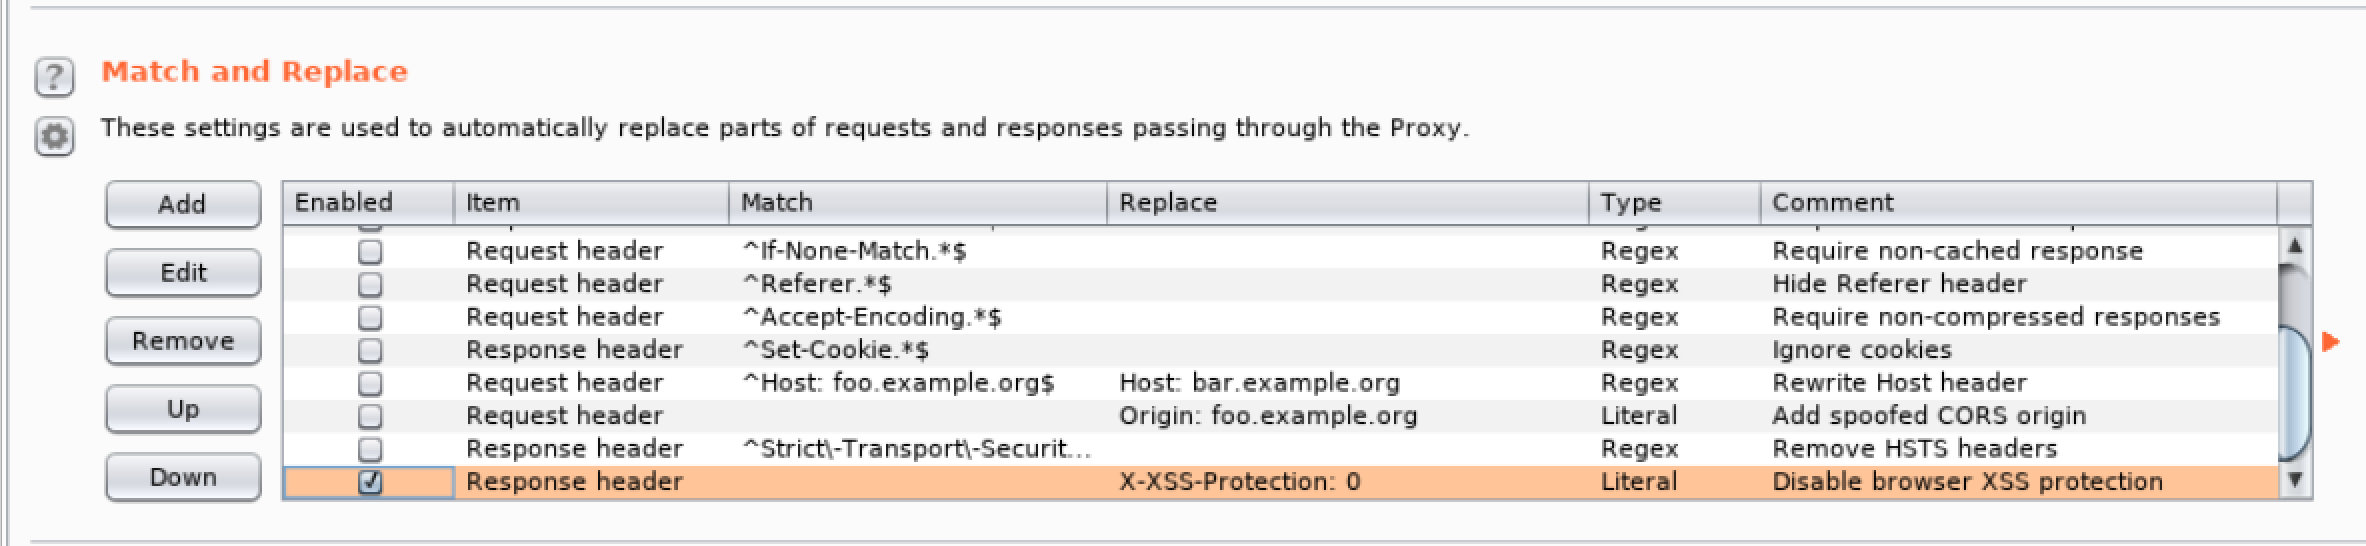
\includegraphics[width=\textwidth]{images/evaluation/burp_xss_disabled.png}
	\caption{Any request passed to Gentoo or the other tools is stripped of the \texttt{X-XSS-Protection} header, allowing for accurate XSS detection.}
	\label{fig:burp_xss_disabled}
\end{figure}

As explained before, we will be extracting 3 key metrics: \textit{Time to Vulnerability}, \textit{Interaction Volume} and \textit{Number of Attacks needed}. \textit{Time to vulnerability} is measured as the time from the moment the scan is initiated until the first 'vulnerability' is detected by the application (irrespective of whether this is the vulnerability we are specifically looking for or not - we will explain the reasoning for this later). \textit{Interaction Volume} is measured as the total number of bytes used in the scan by the tool. \textit{Number of attacks needed} measures how many requests a tool had to make before finding its first vulnerability in the scan (as a proportion to how many requests it made in the scan overall). \\ 

In order to extract data for the purposes of these experiments, we use console logging in Gentoo to acquire accurate timestamps for key events in a scan. For the other tools, we use the provided reporting and exporting functionalities by each tool and analyse the outputs of these to acquire the necessary data. \\

\subsection{Test Harness}

Firstly, we benchmarked the tools against the produced Test Harness. We ran Gentoo using the Action Replay functionality to detect the XSS vulnerabilities present in this page, and subsequently used the Passive Mode to scan the headers in the Test Harness.  \\

\begin{table}[h]
	
{\rowcolors{3}{Apricot}{Wheat1}
	\label{table:test_harness_benchmarks}
	   \captionsetup{justification=centering}
	
	\caption{Running the tools against the Test Harness. The * by the \textit{Time to Vulnerability} column indicates the desired vulnerability (XSS) was not detected}
\begin{tabular}{ |p{4cm}||p{2cm}|p{1.4cm}|p{1.6cm}|p{2cm}|p{2cm}| }
	\hline
	\multicolumn{6}{|c|}{\textbf{Test Harness Benchmarks}} \\ [0.5ex]
	\hline \hline 
	Tool Being Tested& Time To Vulnerability & Total Scan Time & Interaction Volume & Attacks to Vuln / Total Attacks & \% of Scan to 1st Vuln \\
	\hline
	Gentoo (XSS detection)    & 9.6s      & 15.8s    & 32KB & 10/27 &37\% \\
	Gentoo (Header Analysis) & 50ms    &  3.0s    & 4KB&  1/4 &25\%\\
	ZAP                                   & 5.6s (*) & 7.8      &  1.31MB &1621/2140 &76\%\\ 
	w3af                                 & 7.9s  (*) & 136.2s & 950KB & 71/1126 &6.3\%\\
	\hline
\end{tabular}
} \\
\end{table}

The table above describes 

When producing this data, it became evident that comparing Gentoo to these tools on a basis of whether they had found a specific vulnerability on an application seemed unfair. As it stands, our extension is very focused on finding a given vulnerability, and if set up correctly, seems to provide good feedback on said vulnerability. However, ZAP and w3af are stand-alone implementations designed to run without user interaction, and as such, will scan the entire web-application in a non-discriminatory way when it comes to selecting vulnerabilities - anything of use is flagged up for the final report. Thus, although we set up these tests in a manner such that Gentoo \textit{should} find a vulnerability it has been designed to catch, we will not hold it against the results of the other 2 should they find other useful information along the way. \\

In the benchmark above (Table \ref{table:test_harness_benchmarks}), neither ZAP nor w3af reported an XSS vulnerability for the Test Harness. This is perhaps a little odd, as the page containing this vulnerability conforms to the minimum requirements for a Reflected XSS. However, since it is a \textit{very} simple page, it could be supposed that the page is not complex enough for the filters being used to correctly classify an XSS according to the other tools. \\

Nonetheless, all 3 of the tools produced due warnings when \textit{passively} analysing the application, with the exception of w3af, which does not seem to have a separate passive mode. However, when observing the scan outputs, the speed at which these alerts in w3af are produced seems to indicate that internally, these alerts are still acquired passively from webrequests. \\

\begin{table}[h]
	
	{\rowcolors{3}{Apricot}{Wheat1}

		\captionsetup{justification=centering}
		
		\caption{The alerts produced by the different tools when analysing the Test Harness}
				\label{table:test_harness_alerts}
		\begin{tabular}{ |p{8cm}|>{\centering\arraybackslash}m{2cm} |>{\centering\arraybackslash}m{2cm} |>{\centering\arraybackslash}m{2cm}| }
			\hline
			\multicolumn{4}{|c|}{\textbf{Test Harness passive alerts}} \\ [0.5ex]
			\hline \hline 
			Alert Type & Gentoo & ZAP & w3af \\
			\hline
			X-Frame-Options (Clickjacking) & X & X & X \\
			X-XSS-Protection & X & X & \\
			X-Content-Type-Options& X & X & \\
			Content-Security-Policy & X & & \\
			Referrer-Policy & X & & \\
			Strict-Transport-Security & X  & & \\
			Server Header Exposed & & & X\\
			DNS Wildcard config & & & X \\
			Too many HTTP methods allowed & & & X\\
			
			\hline
		\end{tabular}
	} \\
\end{table}

In Table \ref{table:test_harness_alerts}, we see that all of tools can agree that clickjacking is a big enough concern that the \texttt{X-Frame-Options} header should be set. We will ignore the alerts for the missing \texttt{X-XSS-Options} header because this is by design as previously explained, although it is interesting to note that w3af did not report this missing header in its scans. Some of the uniquely reported headers by Gentoo are also more recent additions - both the \texttt{Content-Security-Policy} and the \texttt{Referrer-Policy} are newer headers. As for the last 4 on the Table, these settings are more suggestions than alerts - these are flagged up by Gentoo and w3af, but do not necessarily indicate weaknesses. They are nonetheless useful in the \textit{information gathering} phase of any pentester, and shouldn't be readily ignored.  




\subsection{DVWA}


\begin{table}[h]
	
	{\rowcolors{3}{Apricot}{Wheat1}
		\label{table:dvwa_benchmarks}
		\captionsetup{justification=centering}
		
		\caption{}
		\begin{tabular}{ |p{4cm}||p{2cm}|p{1.4cm}|p{1.6cm}|p{2cm}|p{2cm}| }
			\hline
			\multicolumn{6}{|c|}{\textbf{DVWA Benchmarks}} \\ [0.5ex]
			\hline \hline 
			Tool Being Tested& Time To Vulnerability & Total Scan Time & Interaction Volume & Attacks to Vuln / Total Attacks & \% of Scan to 1st Vuln \\
			\hline
			Gentoo (XSS detection)    & 6.6s      & 9.4s    &   66.3KB          & 4/15 & 27 \% \\
			Gentoo (Header Analysis) & 27ms    &  3.0s    & 17.9KB   &  2/5 & 40\%\\
			ZAP                                  & 2.6s & 66.6s     &  65.79MB & 3852/22995& 16.7\%\\ 
			w3af                                 & -- & -- & -- & -- &-- \\
			\hline
		\end{tabular}
	} \\
\end{table}

\subsection{WebGoat}

bla

\begin{table}[h]
	
	{\rowcolors{3}{Apricot}{Wheat1}
		\label{table:webgoat_benchmarks}
		\captionsetup{justification=centering}
		
		\caption{}
		\begin{tabular}{ |p{4cm}||p{2cm}|p{1.4cm}|p{1.6cm}|p{2cm}|p{2cm}| }
			\hline
			\multicolumn{6}{|c|}{\textbf{WebGoat Benchmarks}} \\ [0.5ex]
			\hline \hline 
			Tool Being Tested& Time To Vulnerability & Total Scan Time & Interaction Volume & Attacks to Vuln / Total Attacks & \% of Scan to 1st Vuln \\
			\hline
			Gentoo (XSS detection)    & --     & --    &   --          & -- & -- \\
			Gentoo (Header Analysis) &  11.6s   & 17.8s   & 52.0KB   & 1/24 & 4.1\%\\
			ZAP                                   & 12.9s &  48.5s   & 68.0MB  & 1213/4437 & 27.3\%\\ 
			w3af                                 & -- & -- & -- & -- & -- \\
			\hline
		\end{tabular}
	} \\
\end{table}

\subsection{WackoPicko}


bla

\begin{table}[h]
	
	{\rowcolors{3}{Apricot}{Wheat1}
		\label{table:wackopicko_benchmarks}
		\captionsetup{justification=centering}
		
		\caption{}
		\begin{tabular}{ |p{4cm}||p{2cm}|p{1.4cm}|p{1.6cm}|p{2cm}|p{2cm}| }
			\hline
			\multicolumn{6}{|c|}{\textbf{WackoPicko Benchmarks}} \\ [0.5ex]
			\hline \hline 
			Tool Being Tested& Time To Vulnerability & Total Scan Time & Interaction Volume & Attacks to Vuln / Total Attacks & \% of Scan to 1st Vuln \\
			\hline
			Gentoo (XSS detection)    &   11.6s   &  17.8s   &  52.0KB           & 1/24 & 4.1\% \\
			Gentoo (Header Analysis) &  51ms &  3.1s  &  1.6KB  & 3/7 & 42.9 \%\\
			ZAP                                   & 53s &  184.3s   & 254.4MB & 10854/46301 & 23.4\%\\ 
			w3af                                 & 458ms & 498s & 7.0MB & 2/8279 & 0.02\% \\
			\hline
		\end{tabular}
	} \\
\end{table}


\section{Live application scanning}


\section{Accessibility}

> Brief introduction to ZAP and w3af, features
> Not being able to scan webgoat
> User feedback
> Being on chrome

> It's clear that gentoo wins because it's already in the browser (which is the best zap feature, not available in w3af making it terrible) 
> Mention the fact i had to disable x-xss-protection maybe renders it a bit useless on sites




































